% !TeX root = ../SDonchezThesis.tex

\chapter{Memory Isolation for Tenant Data Integrity}\label{ch:dmaProtection}
Although the EDF Algorithm outlined in the preceding chapter enables the efficient decryption of tenant bitstreams with shared decryption engines, the encrypted transmission of the bitstream is itself useless if any co-tenant on the PFPGA is granted access to the decrypted bitstream as stored in RAM. To this end, it is imperative that memory isolation functionality be utilized throughout the PFPGA to limit each tenant's partition to only the portions of the memory space that are allocated to said tenant. Similarly, care should be taken to re-allocate access permissions to the decryption engines as they change tasks, such that the end user can be guaranteed that access only persists through the decryption partition for as long as is necessary. Finally, the static partition, containing the CSP's supervisory functionality and resources, should be, to the maximum extent practical, isolated from the tenant data (although the presence of the HPS interface and the DDR controller interface in this region necessitate some amount of unrestricted access).

To this end, the architecture presented in Chapter \ref{ch:systemArchitecture} incorporates the use of Xilinx Memory and Peripheral Protection Units for Programmable Logic Isolation (XMPU-PL), as proposed in \cite{noauthor_memory_2021}. By combining these cores with individual AXI interconnect switches for each partition, and configuring the Region parameters of each core according to the partition it is located in, total isolation can be achieved provided that the static bitstream is from a known and trusted source (as has been outlined elsewhere in this work).

The remainder of this chapter outlines the implementation of this mechanism in the programmable logic. It begins with a discussion of the relevant background material and other academic work in the area. It then outlines in detail the proposed design, and concludes with a discussion of its implementation and the results of testing.

\section{Background}\label{sec:DMABackground}

Many of the academic works that have been published on the topic of multi-tenant FPGA-based systems (such as those discussed in Section \ref{sec:LitImpl} have, at the least, acknowledged the need for memory isolation as a means of ensuring tenant data confidentiality and integrity. Unfortunately, many of these discussions are abstract in nature, and lack concrete implementation. For example, \cite{bag_cryptographically_2020} places the responsibility for memory isolation on the OpenStack architecture they base their design on, without a robust consideration of the application of this isolation to the programmable logic. Meanwhile, \cite{chen_enabling_2014} outlines a detailed plan for memory isolation, but does so by utilizing a processor based virtual environment for each partition, imposing appreciable system overhead while not guaranteeing isolation from malicious cotenants on the programmable logic.

Xilinx, one of the largest FPGA vendors, has furnished several documents discussing the isolation of memory and peripherals in an MPSoC architecture. Their flagship line of MPSoC devices, the Zynq UltraScale+ series, implements a number of Xilinx Memory Protection Units (XMPUs) in conjunction with Xilinx Peripheral Protection Units (XPPUs) to enable the strict isolation of various portions of the system if desired. Figure \ref{fig:XMPPUs} indicates these units within the larger MPSoC architecture, with the XMPU and XPPU cores highlighted in red. \cite{mcneil_isolation_2021} provides a detailed explanation of the use of these units in an MPSoC to afford isolation of domains, as well as a comprehensive discussion of their implementation and limitations.

\begin{figure}[ht]
    \centering
    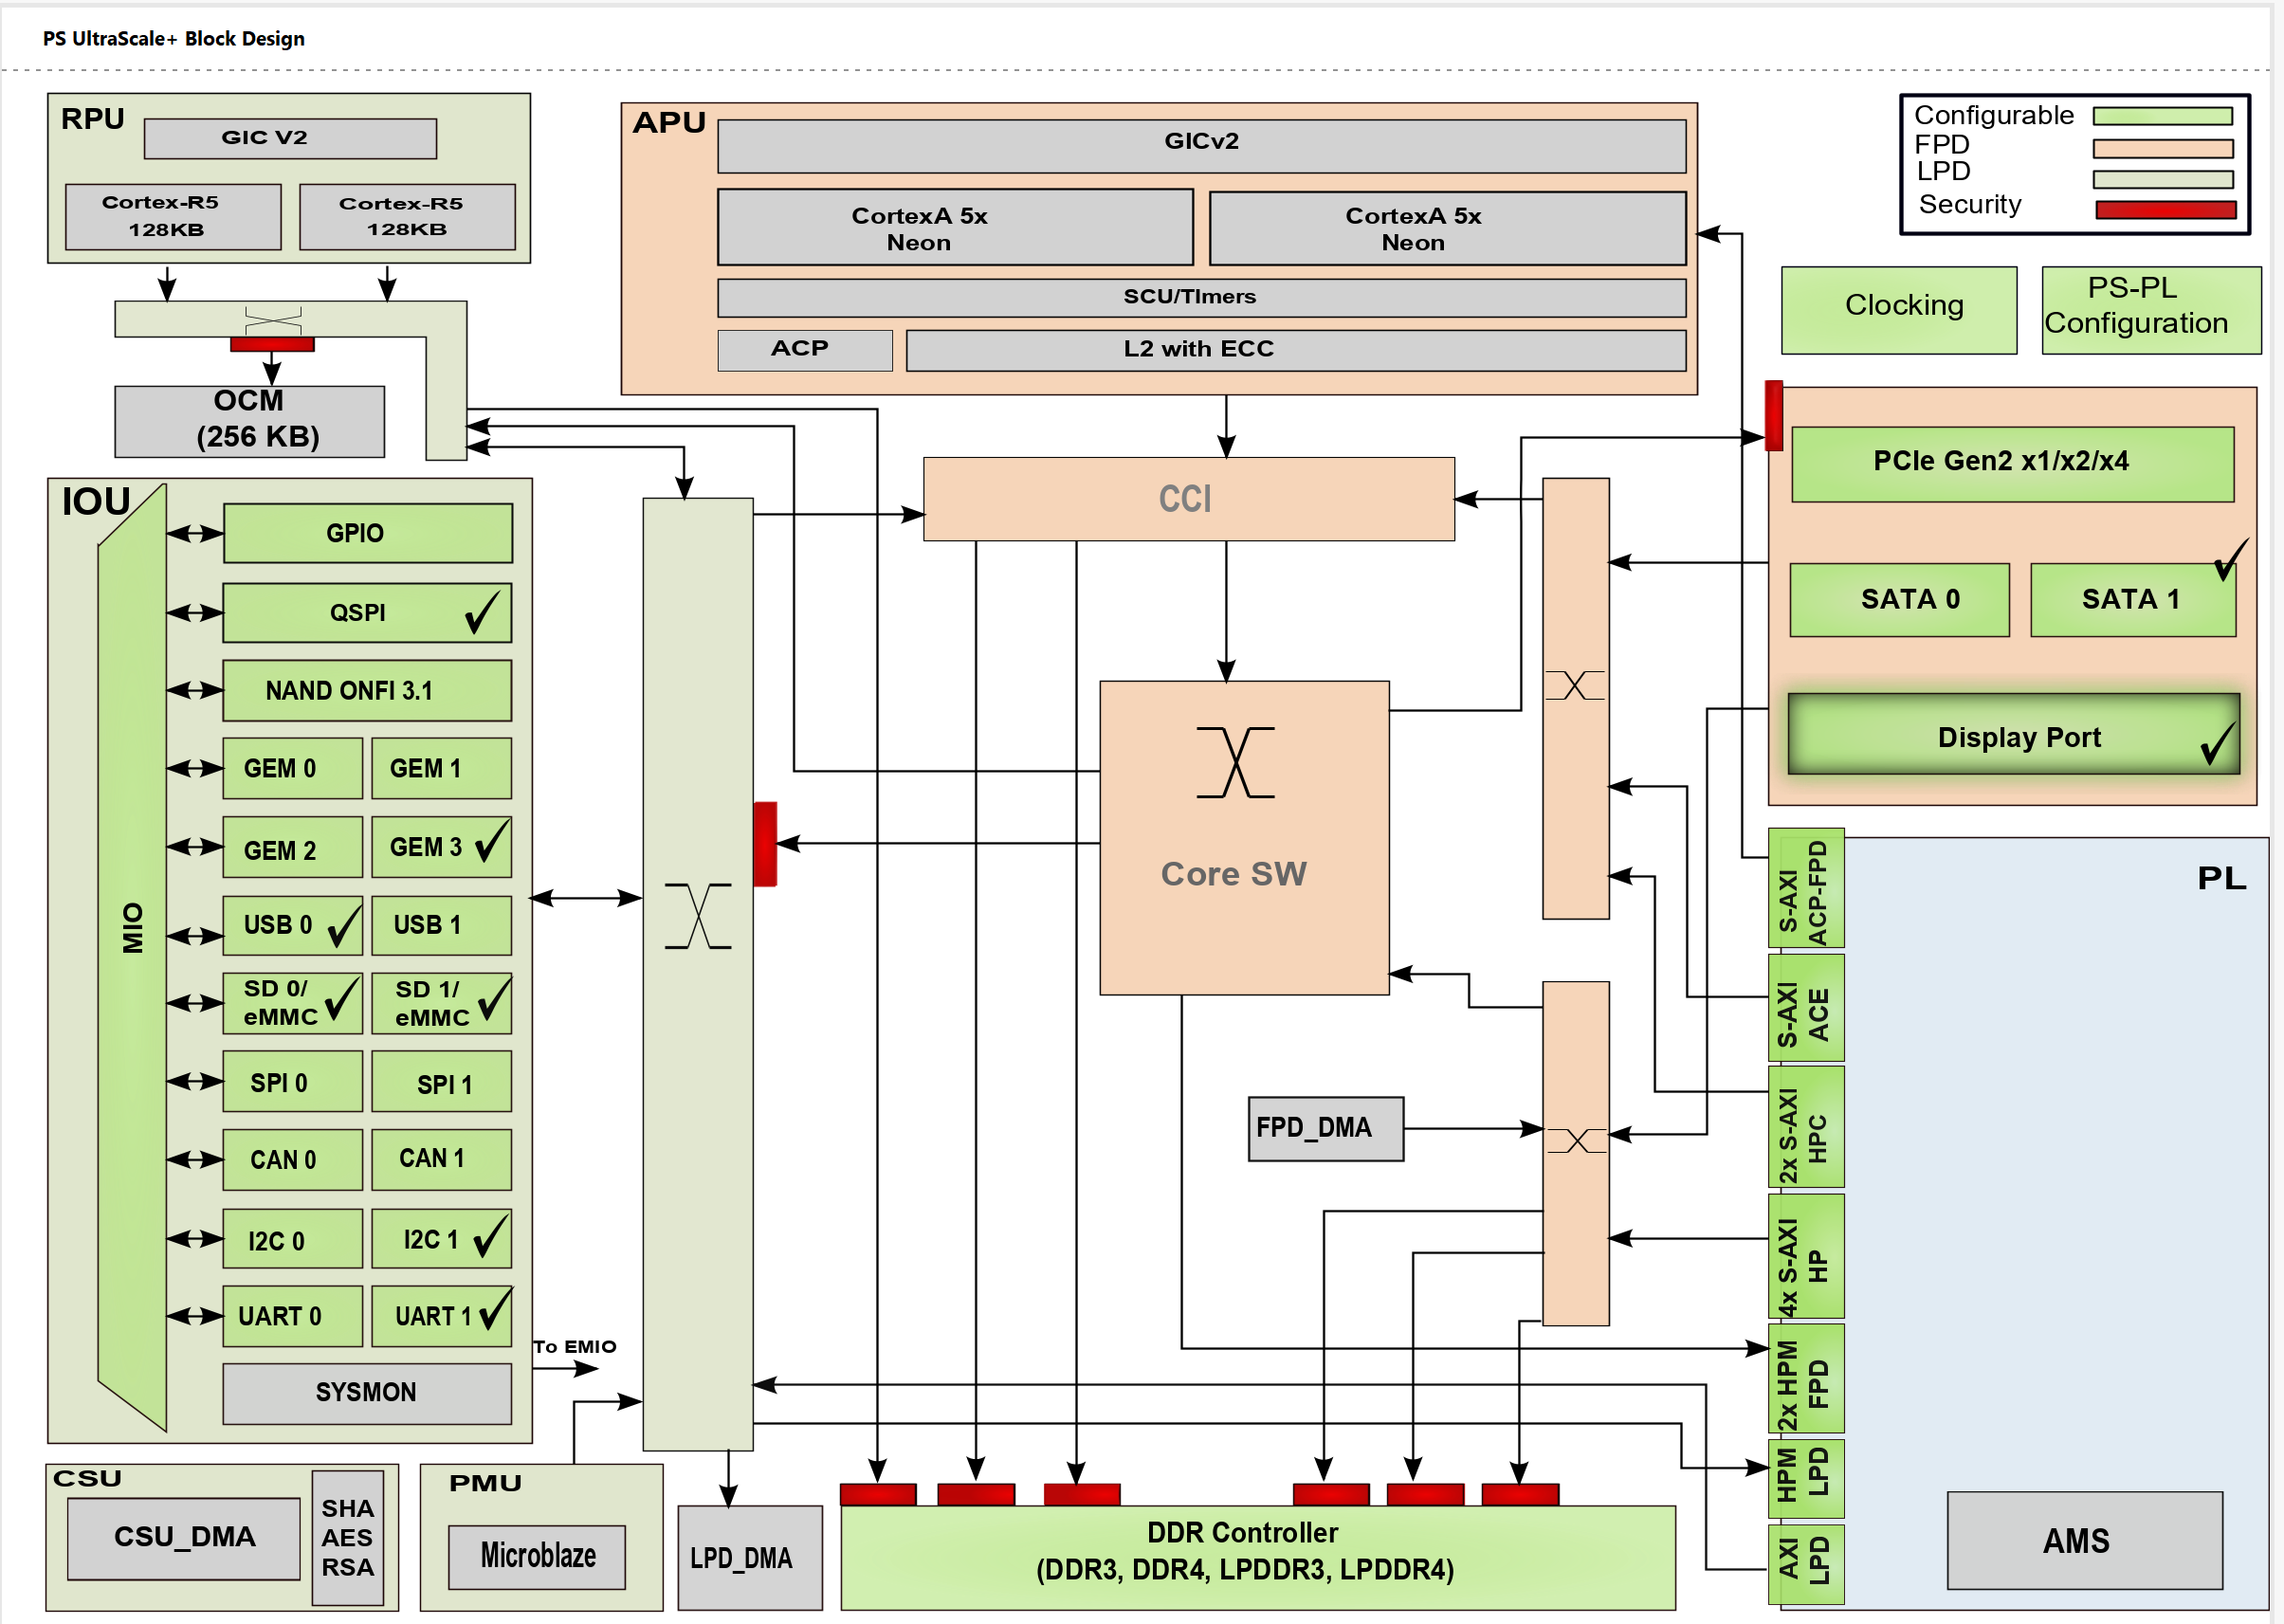
\includegraphics[width=0.8\textwidth]{USP_XMPUs}
    \caption [XMPU and XPPUs in a Zynq UltraScale+]{Xilinx Memory Protection Units (XMPUs) and Xilinx Peripheral Protection Units (XPPUs) within the Zynq UltraScale+ MPSoC architecture}
    \label{fig:XMPPUs}
\end{figure}

As is evident from the figure, these XPPU and XMPU cores are used to enable the isolation of various key portions of the system, including the processors, IO, and various memory devices. However, it is important to note the absence of any isolation functionality within the programmable logic itself, which, tied with the practice of ``memory mapping'' various PL based logic devices, leaves an avenue for malicious co-tenants within the programmable logic to gain access to other tenants' IP. In \cite{noauthor_memory_2021}, Xilinx proposes the aforementioned XMPU-PL IP, which enables the previously absent isolation of memory-mapped PL devices at a granular level. 

This work utilizes these XMPU-PL units to dynamically confine the decryption engines' memory access to whatever tenant partition they are currently processing encrypted bitstream data for (as determined by the scheduling engine outlined in Chapter \ref{ch:edfScheduling}). It also utilizes the XMPU-PLs to serve as a ``gate'' for all memory requests for each partition, thereby preventing a malactor from attempting to access other tenants' devices or memory space.

\section{Proposed Memory Isolation Design}\label{sec:DMADesign}

The memory isolation scheme proposed by this research effort is depicted in Figure \ref{fig:XMPU-PLDesign}, and presented enlarged as Appendix \ref{apx:xmpu-pl-design-enlarged}. As can be seen in the figure, the PL is laid out in a star-like design, with the processor interface (through which the various partitions are administered) at its core. Data from the processor interface is directed through an interconnect IP, which acts as a crossbar switch to route data to the appropriate target. From this interconnect, data flows through one of a series of XMPU-PL units, one per partition, before entering a second interconnect from which data is distributed within the partition. In this way, data is free to flow between devices within a partition (over this internal interconnect), but all requests to external resources are constrained to the partition's memory space by the XMPU-PL. Meanwhile, access to the various management ports is routed directly to the PS interface, preventing malicious co-tenants from attempting to control these resources.
\begin{figure}[ht]
    \centering
    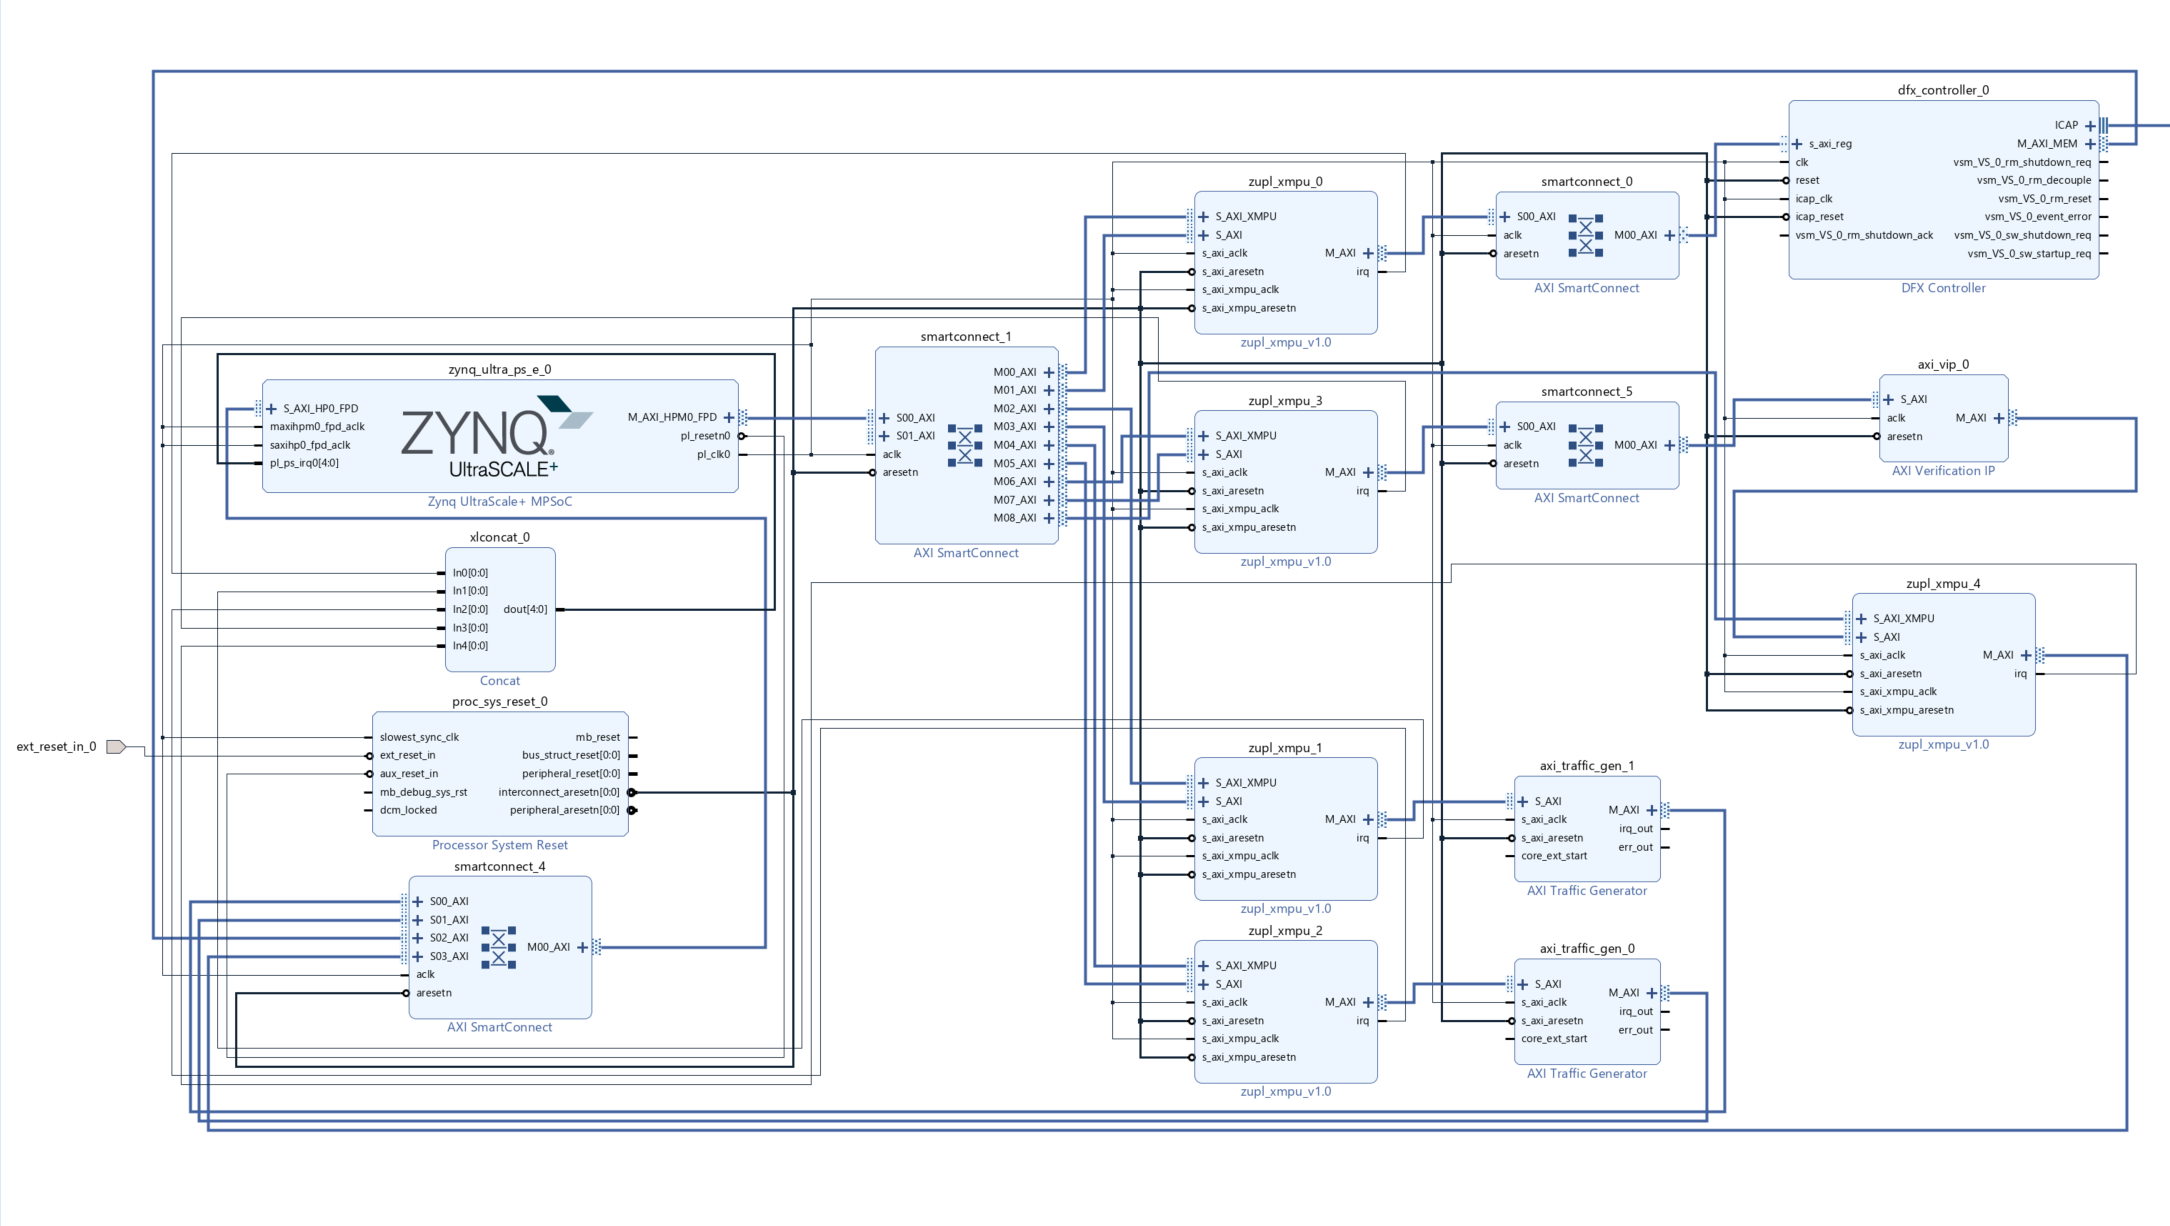
\includegraphics[width=\textheight, angle=90]{isolation_bd.png}
    \caption [Proposed XMPU-PL Design]{Xilinx Memory Protection Unit for Programmable Logic (XMPU-PL) in a Zynq UltraScale+ MPSoC architecture}
    \label{fig:XMPU-PLDesign}
\end{figure}

It should be acknowledged that the block diagram presented in Figure \ref{fig:XMPU-PLDesign} is necessarily simplified from what an actual CSP's implementation would afford. For starters, the design utilizes a pair of AXI-Data Stream FIFO (First in First Out) cores as stand-ins for a KAC engine and an AES engine, respectively. This is to enable a focus specifically on the memory isolation in this design, as opposed to attempting to implement a full architecture. Additionally, it should be noted that this design only implements a single AES-representative FIFO, and similarly only a single Dynamic Reconfiguration Controller, where a more realistic implementation would include several AES engines (per the scheduler outlined in Chapter \ref{ch:edfScheduling}, above), as well as a separate Dynamic Partial Reconfiguration controller for each tenant partition. Finally, it should be noted that the use of AXI-Memory Mapped to Stream converters, seen in the right side of the image, is specific to the implementation of the FIFOs as stand-in cores, and may not be necessary for the actual implementation of the design with decryption cores instead of FIFOs.
\section{Development and Test Environment}\label{sec:DMAEnvironment}

\subsection{Development Environment}\label{subsec:DMAEnvironmentDev}
The design presented in \ref{fig:XMPU-PLDesign} was implemented utilizing the same developer machine as outlined in \ref{subsec:devEnv}. Specifically, the development machine used by the authors in the course of this project was a Windows 10 Professional Edition 64-bit laptop featuring an Intel Core i7-9750H CPU with a base frequency of 2.60GHz. The machine featured 16 GB of DDR4 DRAM and a 1 TB SSD. Furthermore, the build process utilized the same Docker container as outlined in \ref{subsec:devEnv} to facilitate the development of the design.

\subsection{Target Hardware}\label{subsec:DMAEnvironmentHW}
Unlike the previous design, the desired use of the UltraScale+ architecture, with all of the isolation benefits outlined above, required the transition of the research effort away from the use of the ZedBoard as a hardware platform of choice. Instead, this effort targeted a recently released development platform that provides an affordable UltraScale+ MPSoC system, the Alinx AXU2CGB. The AXU2CGB, depicted in Figure \ref{fig:AXU2CGB}, is a compact development platform that includes an XCZU2CG-1SFVC784E UltraScale+ MPSoC. This MPSoC integrates a Dual-Core ARM Cortex-A53 Application Processor with a Dual-Core ARM Cortex-R5 Real Time Processor, combined with an FPGA that boasts over 103,000 logic cells, 94,000 look up tables, 240 DSP slices, 5.3 Mb of Block RAM, and 32MB of QSPI Flash. The larger AXU2CGB board also provides 2 GB of DDR4 RAM, as well as an 8GB EMMC Flash device.

\begin{figure}
    \centering
    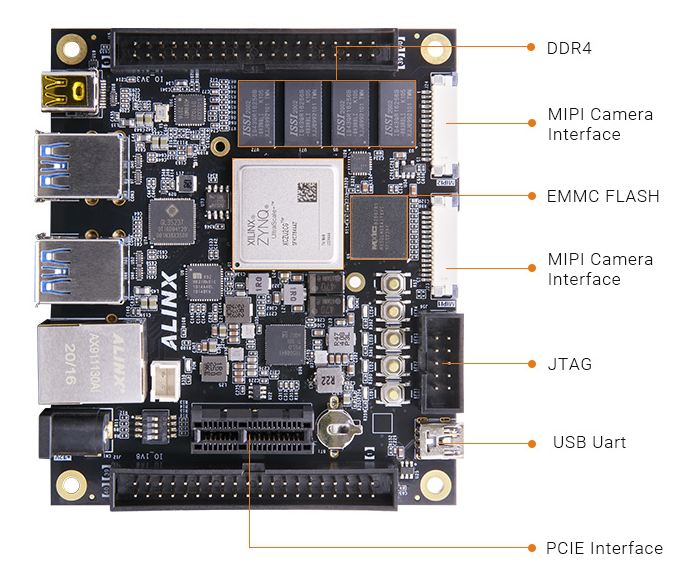
\includegraphics[]{axu2cgb.png}
    \caption[AXU2CGB Development System]{Alinx AXU2CGB Development System, with key components highlighted \cite{noauthor_axu2cgb_nodate}}
    \label{fig:AXU2CGB}
\end{figure}

\subsection{Target Operating System}\label{subsec:DMAEnvironmentOS}
Much like the ZedBoard, the AXU2CGB is well suited for the PetaLinux operating environment provided by Xilinx for use on its SoCs. Initial efforts targeting this board have utilized the stock PetaLinux image provided with the purchase of the board, which is based on the same PetaLinux 2020.2 toolchain as previously discussed. Later efforts implementing various test applications have utilized slightly modified variants, which are discussed in subsequent sections. Additionally, certain tests were conducted in a ``bare-metal'' environment, wherein the applications were executed directly on the target without an operating system serving as a middle layer.

\section{Implementation and Experimental Results}\label{sec:DMAResults}
One immediate takeaway from the implementation of the design shown in \ref{fig:XMPU-PLDesign}, above, is that it consumes a large portion of the available PL, even on a recent (and comparatively large) FPGA such as the one afforded by the AXU2CGB. As the utilization report shown in Figure \ref{fig:XMPU-PLUtilization} shows, nearly 75\% of all Look Up Tables (LUTs) are consumed in this design. However, it should be noted that such an FPGA is appreciably smaller still than the large format devices that will likely become the tool of choice for cloud based operations, and in such instances this design yields appreciable savings over the previously proposed architectures.

\begin{figure}
    \centering
    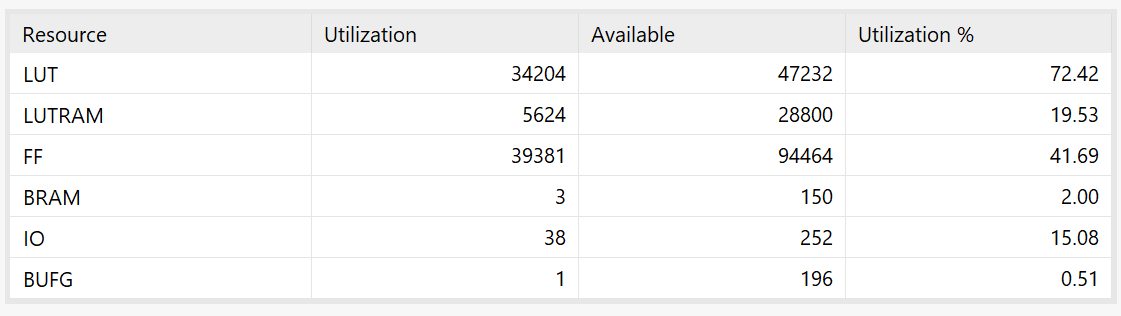
\includegraphics[width=0.8\textwidth]{xmpupl_utilization.png}
    \caption[Memory Isolation Resource Utilization]{Resource Utilization for the XMPU-PL design, as implemented on the AXU2CGB}
    \label{fig:XMPU-PLUtilization}
\end{figure}